%!TEX root = ../thesis.tex
% створюємо розділ
\chapter{Огляд моделей машинного навчання навчання та функцій втрат}
\label{chap:theory}

\section{Модель Feature Pyramid Networks}

FPN (Feature Pyramid Networks) -- це інструмент для виділення ознак, який
приймає на вхід одномасштабне зображення довільного розміру, а на вихід подає
карти ознак пропорційного розміру на декількох рівнях, повністю згорнуті за
допомогою методу згортки~\cite{lin2016}. Цей процес не залежить від базової
згорткової архітектури. Тому він діє як загальне рішення для побудови пірамід
ознак всередині глибоких згорткових мереж для використання в таких задачах, як
виявлення об'єктів.

FPN -- це передова архітектура, яка широко використовується в задачах
комп'ютерного зору, зокрема, для виявлення та сегментації об'єктів. Архітектура
FPN вирішує проблему виявлення об'єктів різного масштабу шляхом створення
різномасштабного представлення ознак з одного вхідного зображення. Це
досягається за допомогою ієрархічного підходу, який використовує властиву
згортковим нейронним мережам (CNN) форму піраміди. Основна ідея полягає в тому,
щоб будувати карти об'єктів з різною роздільною здатністю, фіксуючи дрібні
деталі з високою роздільною здатністю і більш абстрактні об'єкти з низькою
роздільною здатністю, що дозволяє надійно виявляти об'єкти різного розміру.

Загальна архітектура мереж FPN зображена на рис.~\ref{fpn_arch}. FPN складається з двох основних частин: висхідного шляху та низхідного шляху з
бічними зв'язками. Висхідний шлях -- це стандартна згорткова мережа, яка
створює карти ознак з меншою просторовою роздільною здатністю, але більшою
семантичною насиченістю. Шлях згортання зверху-вниз потім підвищує
дискретизацію цих карт ознак для створення піраміди ознак з вищою роздільною
здатністю. Бічні зв'язки використовуються для об'єднання об'єктів з висхідного
шляху з вибіркою об'єктів з низхідного шляху, покращуючи представлення кожного
рівня в піраміді. Цей процес об'єднання поєднує семантичну інформацію з глибших
шарів з просторовою інформацією з більш дрібних шарів, в результаті чого
створюються карти об'єктів, які є як семантично сильними, так і просторово
точними. FPN довели свою високу ефективність у підвищенні продуктивності різних
систем виявлення об'єктів, таких як Faster R-CNN і Mask R-CNN, забезпечуючи
багатші і більш дискримінативні представлення ознак для виявлення
різномасштабних об'єктів.

\begin{figure}[ht]
    \centering
    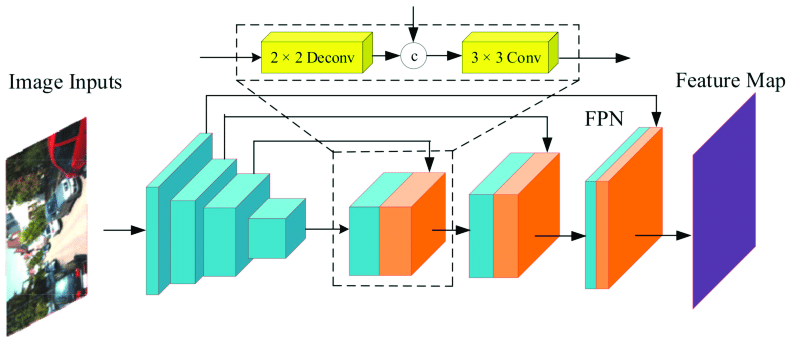
\includegraphics[scale=0.5]{Images/fpn_arch.png}
    \caption{Архітектура мереж FPN}
    \label{fpn_arch}
\end{figure}

FPN суттєво вплинули на різні реальні застосування, особливо в галузях, що
вимагають високоточного виявлення та сегментації об'єктів. В автономному
водінні FPN відіграють вирішальну роль в ідентифікації об'єктів, таких як
пішоходи, транспортні засоби та дорожні знаки, на основі зображень, отриманих з
камер, встановлених на транспортних засобах~\cite{liao2021}. Багатомасштабне
представлення об'єктів дозволяє з високою точністю виявляти як дрібні об'єкти,
такі як віддалені пішоходи, так і великі, наприклад, транспортні засоби, що
знаходяться поблизу. Ця можливість є життєво важливою для безпеки та надійності
автономних систем, де детальне розуміння навколишнього середовища має важливе
значення для навігації та прийняття рішень.

Загалом, універсальність та ефективність
Feature Pyramid Networks роблять їх потужним
інструментом у багатьох галузях, сприяючи
технологічному прогресу та підвищуючи точність
і надійність різних застосувань.

\section{Модель U-Net}

U-Net -- це архітектура згорткової нейронної мережі, розроблена в першу чергу
для біомедичної сегментації зображень. Представлена у
роботі~\cite{ronneberger2015}, U-Net набула значної популярності завдяки своїй
видатній продуктивності в різних задачах сегментації зображень. Архітектура
отримала назву <<U-Net>> через свою характерну U-подібну структуру, яка
складається зі шляху, що звужується (енкодер), і шляху, що розширюється
(декодер). Така конструкція дозволяє U-Net фіксувати як контекст, так і точну
локалізацію, що робить її особливо ефективною для сегментації невеликих і
складних структур на зображеннях (рис.~\ref{unet_arch}).

\begin{figure}[ht]
    \centering
    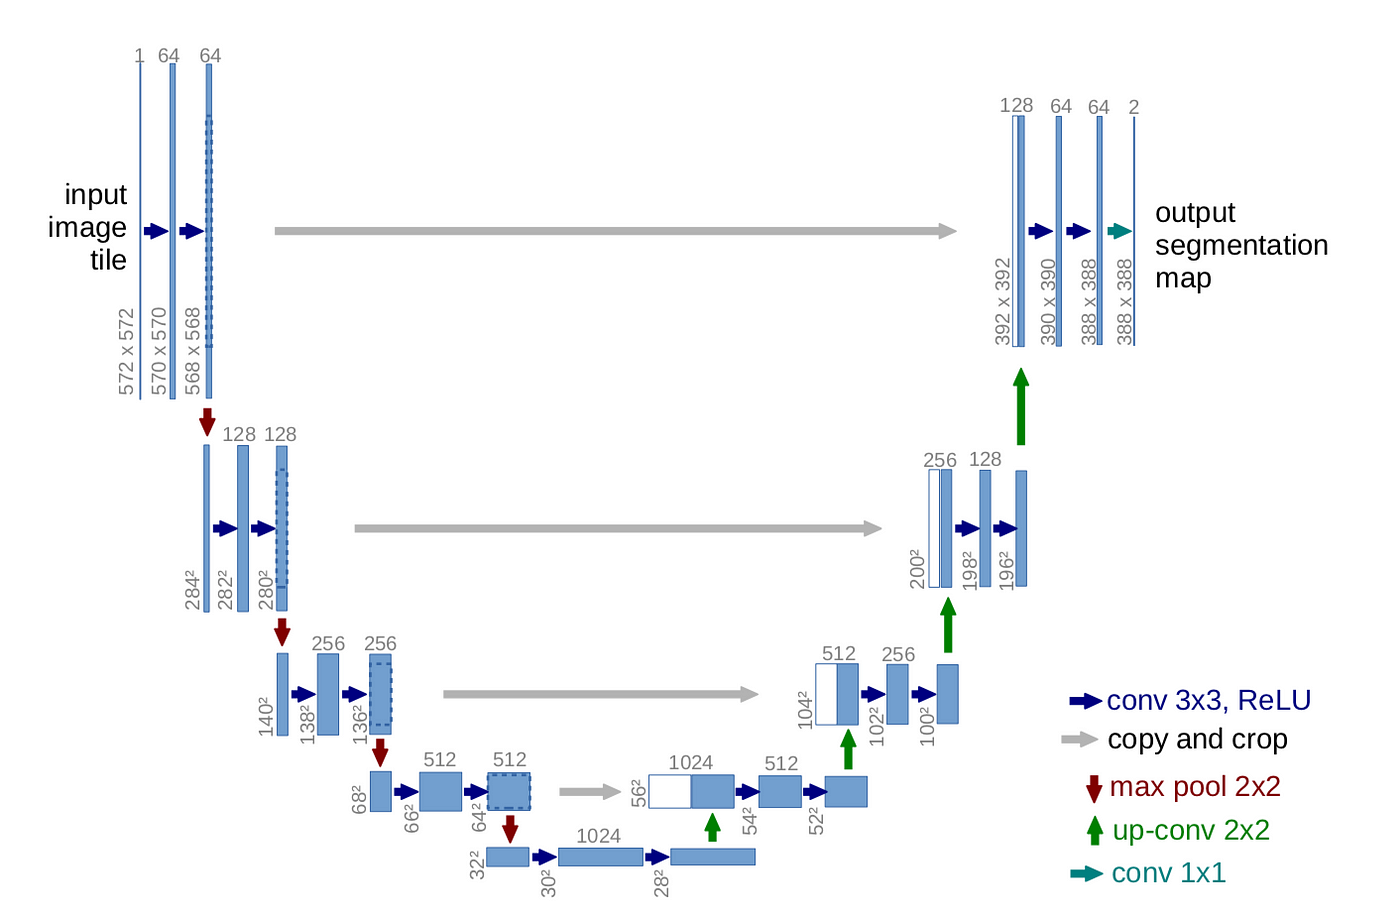
\includegraphics[scale=0.3]{Images/unet_arch.png}
    \caption{Архітектура U-Net}
    \label{unet_arch}
\end{figure}

Шлях згортання U-Net відповідає структурі типової згорткової
мережі, що складається з багаторазового застосування
згорткових шарів, за кожним з яких слідує активація
випрямленої лінійної одиниці (ReLU) та операція
максимального об'єднання для подальшої дискретизації.
Така послідовність операцій зменшує просторові розміри
карт ознак, одночасно збільшуючи їхню глибину,
що дозволяє мережі вивчати ієрархічні ознаки на різних
масштабах. Кожен крок на шляху звуження фіксує все
більш абстрактні представлення вхідного зображення,
які мають вирішальне значення для розуміння складних
закономірностей і контексту.

Розширювальний шлях є дзеркальним відображенням звужувального
шляху, але виконує протилежні операції. Він передбачає
збільшення вибірки карт об'єктів, зазвичай за допомогою
транспонованих згорток (також відомих як деконволюції),
для збільшення їхньої просторової роздільної здатності.
На кожному кроці збільшення вибірки мережа об'єднує
відповідні карти ознак зі шляху скорочення за допомогою
пропускних зв'язків. Ці з'єднання відіграють життєво
важливу роль в архітектурі U-Net, зберігаючи об'єкти з
високою роздільною здатністю, які в іншому випадку були
б втрачені під час процесу пониження дискретизації.
Поєднуючи ці детальні характеристики з високорівневою
семантичною інформацією, отриманою з глибших шарів,
мережа може точно окреслити межі об'єктів на зображенні.

Загалом, архітектура U-Net дозволяє ефективно
балансувати між необхідністю детальної локалізації
та контекстним розумінням, що робить його високоефективним
для задач сегментації зображень. Інноваційне використання
пропускних з'єднань і симетричний дизайн зробили її
популярним вибором у різних галузях, окрім біомедичної
візуалізації, включаючи аналіз супутникових зображень,
сільськогосподарський моніторинг тощо, де точна
сегментація має вирішальне значення.

U-Net знайшла широке застосування в різних галузях реального світу, а її
основні історії успіху пов'язані з біомедичною візуалізацією. У медичній
діагностиці U-Net використовується для сегментації анатомічних структур на
радіологічних зображеннях, таких як МРТ і КТ. Її здатність точно окреслювати
межі органів, тканин і патологічних ділянок, таких як пухлини, робить її
безцінною для допомоги радіологам у діагностиці та плануванні лікування.
Наприклад, в онкології U-Net допомагає ідентифікувати і вимірювати об'єм
пухлини, що має вирішальне значення для оцінки прогресування раку і планування
відповідних втручань.

Окрім медичної візуалізації, U-Net була успішно адаптована
для використання в екологічному і сільськогосподарському
моніторингу за допомогою аналізу супутникових і аерофотознімків
У цих сферах U-Net допомагає сегментувати різні типи
земного покриву, такі як ліси, міські території і водні
об'єкти, на основі супутникових знімків. Ця інформація
має вирішальне значення для моніторингу змін навколишнього
середовища, управління природними ресурсами і планування
міського розвитку. Крім того, в землеробстві U-Net
використовується для аналізу стану посівів шляхом сегментації
різних типів рослинності та виявлення ділянок, уражених
хворобами чи шкідниками~\cite{mou2018}. Ця програма дозволяє фермерам
здійснювати цілеспрямовані втручання, тим самим підвищуючи
врожайність і зменшуючи використання пестицидів.

\section{Модель DeepLabv3}

DeepLabv3~\cite{chen2017} -- це сучасна модель глибокого навчання для
семантичної сегментації зображень, яка полягає в поділі зображення на регіони
та визначенні категорії об'єктів, присутніх у кожному регіоні. Розроблена
Google Research, DeepLabv3 базується на попередніх версіях, DeepLabv1 і
DeepLabv2, і включає в себе кілька ключових інновацій, які підвищують її
продуктивність і точність. Одним з головних досягнень DeepLabv3 є використання
технології atrous convolution (також відомої як розширена згортка), яка
дозволяє ефективно збільшувати рецептивне поле без втрати роздільної здатності.
Ця методика дозволяє моделі захоплювати різномасштабну контекстну інформацію,
що має вирішальне значення для точної сегментації об'єктів різного розміру.

Ще однією важливою особливістю DeepLabv3 є використання
atrous spatial pyramid pooling (ASPP).
ASPP застосовує atrous convolution з різною швидкістю розширення
паралельно для захоплення інформації на різних масштабах. Цей
механізм вилучення різномасштабних ознак покращує здатність моделі
розпізнавати об'єкти на різних рівнях деталізації та просторових вимірів.
Крім того, DeepLabv3 інтегрує пакетну нормалізацію, яка стабілізує
і прискорює процес навчання шляхом нормалізації вхідних шарів.
Ця модель може бути реалізована з різними наперед тренованими енкодерами,
такими як ResNet, що ще більше підвищує її продуктивність
і адаптивність до різних завдань і наборів даних.

Крім того, модуль ASPP у DeepLabv3 ефективно фіксує різномасштабну
інформацію, досліджуючи особливості за допомогою фільтрів з
різними частотами дискретизації та полями зору. Експериментальні
результати моделі демонструють значні покращення порівняно з
попередніми версіями, досягнувши продуктивності 85,7\% на тестовому
наборі PASCAL VOC 2012 без необхідності постобробки DenseCRF.

DeepLabv3 є значним досягненням у галузі семантичної сегментації зображень,
пропонуючи надійну продуктивність і високу точність у різних додатках.
DeepLabv3 ефективно фіксує різномасштабну контекстну інформацію, що має
вирішальне значення для сегментації об'єктів різного розміру та складності.
Інтеграція пакетної нормалізації ще більше стабілізує процес навчання,
підвищуючи ефективність та надійність моделі.

\section{Функція втрат Dice Loss}

Dice Loss -- це популярна функція втрат, яка використовується переважно в
галузі сегментації зображень, особливо в аналізі медичних
зображень~\cite{zhang2021}. Вона походить від коефіцієнта Сьоренсена-Дайса,
статистичної міри, яка кількісно оцінює схожість між двома наборами. Dice Loss
особливо ефективна для задач, де набір даних незбалансований, наприклад, для
сегментації невеликих структур, таких як пухлини на медичних зображеннях.
Основною перевагою Dice Loss є його здатність впоратися з таким дисбалансом,
безпосередньо максимізуючи перекриття між прогнозованою сегментацією і базовою
істиною, що має вирішальне значення для отримання точних результатів
сегментації.

Математично коефіцієнт Дайса визначається як подвоєна
площа перекриття між прогнозованою сегментацією
і базовим зображенням, поділена на загальну кількість
пікселів на обох зображеннях. В контексті сегментації
зображень, втрати Дайс формулюються як одиниця мінус
коефіцієнт Дайс, який перетворює міру схожості у
функцію втрат, яку можна мінімізувати. Формулу для
Dice Loss можна записати як:

\begin{equation*}
    DL = 1 - \frac{2|A \cap B|}{|A| + |B|},
\end{equation*}
де A -- набір пікселів у прогнозованій сегментації,
а B -- набір пікселів у істинній сегментації.
Мінімізуючи Dice Loss, модель заохочується
до максимізації перекриття між прогнозованою
та фактичною сегментацією, таким чином покращуючи
точність сегментації.

Включення Dice Loss у процес навчання дозволяє моделі
навчитися вловлювати складні просторові взаємозв'язки
та дрібні деталі, присутні на супутникових знімках,
що призводить до більш точних результатів сегментації.

Крім того, використання Dice Loss допомагає
пом'якшити дисбаланс класів, який часто зустрічається
в задачах сегментації супутникових знімків. Супутникові
знімки зазвичай містять великі ділянки однорідного фону,
що перемежовуються з меншими регіонами, які становлять
інтерес. Dice Loss вирішує цю проблему,
призначаючи вищі штрафи за неправильну
класифікацію класів меншин, тим самим сприяючи
збалансованій сегментації різних типів земного покриву.
Загалом, інтеграція Dice Loss для
сегментації супутникових знімків підвищує
здатність моделей машинного навчання видобувати значущу
інформацію з супутникових знімків, полегшуючи різні
подальші застосування в таких галузях, як моніторинг
довкілля, сільське господарство і міське планування.

\section{Функція втрат Focal Loss}

Focal Loss -- це функція втрат, запропонована в роботі~\cite{lin2017} для
усунення екстремального дисбалансу класів, що виникає під час навчання
детекторів щільних об'єктів. Цей дисбаланс виникає, коли в наборі даних значно
більше простих негативних прикладів, ніж позитивних. Focal Loss має на меті
зменшити втрати, пов'язані з добре класифікованими прикладами, і зосередити
навчання на важких, неправильно класифікованих прикладах. Це досягається
додаванням модулюючого множника $(1 - p_t)^\gamma$ до стандартної перехресної
ентропійної втрати (cross-entropy loss), де $p_t$ представляє прогнозовану
ймовірність класу базової істини, а $\gamma \geq 0$ -- фокусний параметр.

Таким чином, формула для Focal Loss має наступний вигляд:

\begin{equation*}
    FL(p_t) = -(1-p_t)^\gamma log(p_t).
\end{equation*}

Основна ідея Focal Loss полягає в тому,
щоб зменшити внесок простих прикладів під час навчання,
таким чином запобігаючи їхньому перевантаженню датчика.
Регулюючи параметр фокусування $\gamma$, можна контролювати швидкість,
з якою легкі приклади втрачають вагу. Коли приклад
невірно класифіковано і $p_t$ малий, модулюючий коефіцієнт близький до
1, і втрати не впливають. Однак, коли $p_t$ наближається до 1,
коефіцієнт зменшується до 0, що призводить до зменшення втрат
для добре класифікованих прикладів.

Focal Loss призначена для обробки дисбалансу класів безпосередньо через функцію
втрат, на відміну від традиційних методів, таких як двоступеневі детектори, які
покладаються на каскадні механізми і зміщену вибірку. Зосереджуючись на важких
негативних прикладах, Focal Loss дозволяє ефективно навчати на всіх прикладах
без необхідності вибірки або схем перезважування.

Експериментальні результати, представлені в роботі~\cite{lin2017},
демонструють ефективність Focal Loss у навчанні високоточного
одноетапного детектора об'єктів під назвою RetinaNet.
Focal Loss перевершує попередні методи боротьби з дисбалансом класів,
такі як евристика вибірки або навчання на складних прикладах,
і дозволяє детектору досягти кращої точності, зберігаючи при цьому швидкість.

\subsection*{Висновки до розділу 2}
Отже, у даному розділі було проведено огляд моделей машинного навчання
та функцій втрат. Було досліджено три сучасні архітектури мереж: FPN, U-Net, та DeepLabv3 які вже
тривалий час показують свою ефективність у задачах сегментації зображень,
в основному, на медичних знімках. Досліджуваними функціями втрат були
Dice Loss і Focal Loss, які теж часто використовується у задачах сегментації. У ході
дослідження було виявлено, що дані інструменти гарно підійдуть для
сегментації кратерів на супутникових знімках.